\documentclass[a4paper,11pt]{article}

% - Essential Packages -
\usepackage[utf8]{inputenc}
\usepackage[english]{babel}
\usepackage{geometry}
\geometry{margin=1in}
\usepackage{parskip}
\usepackage{setspace}
\usepackage{listings}
\usepackage{upquote}
\usepackage{xcolor}
\usepackage{graphicx}
\usepackage{booktabs}
% Float positioning control (figures/tables)
\usepackage{float}            % allows using [H] to force the figure in place
\usepackage[section]{placeins} % prevents floats from crossing \section boundaries
% Package for links in the table of contents and references
\usepackage[colorlinks=true, linkcolor=black, urlcolor=blue]{hyperref}

\setstretch{1.2}

% - SQL Code Configuration -
\lstset{
    language=SQL,
    basicstyle=\ttfamily\small,
    keywordstyle=\color{blue},
    commentstyle=\color{gray},
    stringstyle=\color{red},
    breaklines=true,
    frame=single,
    showstringspaces=false,
    columns=fullflexible,
    keepspaces=true
}

% - Cover Information -
\title{
    \vspace{2cm}
    \textbf{\huge Data Administration in Information Systems} \\
    \vspace{1cm}
    \Large Project Report -- 2025/2026 \\
    \vspace{0.5cm}
}
\author{
    \textbf{Rodrigo Perestrelo - ist1106074} \\ \textbf{João Santos - ist1107365}
}
\date{\vfill \today}

\begin{document}

% - 1. Cover Page -
\maketitle
\thispagestyle{empty} % Remove page number from cover
\newpage

% - 2. Table of Contents -
\pagenumbering{roman} % Roman numerals for the table of contents
\tableofcontents
\newpage

% - 3. Main Content -
\pagenumbering{arabic} % Reset numbering to arabic (1, 2, 3...)
\setcounter{page}{1}

\section{Task 1: Table Creation and Data Insertion}

In this task, the storage tables were created and data from CSV files was loaded.

The tables \texttt{ShortPricePaidData2024} and \texttt{ShortPricePaidData2025} were created with the 12 columns specified in the assignment, including integrity constraints (\texttt{CHECK}) to validate \texttt{PropertyType} and \texttt{OldNew}:

\begin{lstlisting}[caption=Main tables creation]
CREATE TABLE ShortPricePaidData2024 (
    TransactionID UNIQUEIDENTIFIER DEFAULT NEWID(),
    Price MONEY NOT NULL,
    DateOfTransfer DATETIME NOT NULL, 
    Postcode VARCHAR(10),
    PropertyType CHAR(1) NOT NULL,
    OldNew CHAR(1) NOT NULL,
    PAON VARCHAR(60) NOT NULL,
    Street VARCHAR(60),
    Locality VARCHAR(40),
    Town VARCHAR(40),
    District VARCHAR(40),
    County VARCHAR(40),
    
    CONSTRAINT CK_PropertyType CHECK (PropertyType IN ('D', 'S', 'T', 'F', 'O')),
    CONSTRAINT CK_OldNew CHECK (OldNew IN ('Y', 'N'))
);

CREATE TABLE ShortPricePaidData2025 (
    TransactionID UNIQUEIDENTIFIER DEFAULT NEWID(),
    Price MONEY NOT NULL,
    DateOfTransfer DATETIME NOT NULL, 
    Postcode VARCHAR(10),
    PropertyType CHAR(1) NOT NULL,
    OldNew CHAR(1) NOT NULL,
    PAON VARCHAR(60) NOT NULL,
    Street VARCHAR(60),
    Locality VARCHAR(40),
    Town VARCHAR(40),
    District VARCHAR(40),
    County VARCHAR(40)
);
\end{lstlisting}

\subsection{Data Insertion via BULK INSERT}

Since the CSV files contain 16 columns in total (including fields such as \texttt{Duration}, \texttt{SAON}, \texttt{PPD\_Category} and \texttt{Record\_Status} that are not required), the following strategy was adopted: Create a \textit{staging} table with all CSV columns, load the file using \texttt{BULK INSERT}, copy only the 12 relevant columns into the final table, and drop the \textit{staging} table.


\begin{lstlisting}[caption=Complete insertion pipeline (example for 2024)]
-- Phase 1: Staging table with full CSV structure
CREATE TABLE PricePaidData2024 (
    TransactionID UNIQUEIDENTIFIER,
    Price MONEY,
    DateOfTransfer DATETIME,
    Postcode VARCHAR(10),
    PropertyType CHAR(1),
    OldNew CHAR(1),
    Duration CHAR(1),
    PAON VARCHAR(60),
    SAON VARCHAR(40),
    Street VARCHAR(60),
    Locality VARCHAR(40),
    Town VARCHAR(40),
    District VARCHAR(40),
    County VARCHAR(40),
    PPD_Category CHAR(1),
    Record_Status CHAR(1)
);

CREATE TABLE PricePaidData2025 (
    TransactionID UNIQUEIDENTIFIER,
    Price MONEY,
    DateOfTransfer DATETIME,
    Postcode VARCHAR(10),
    PropertyType CHAR(1),
    OldNew CHAR(1),
    Duration CHAR(1),
    PAON VARCHAR(60),
    SAON VARCHAR(40),
    Street VARCHAR(60),
    Locality VARCHAR(40),
    Town VARCHAR(40),
    District VARCHAR(40),
    County VARCHAR(40),
    PPD_Category CHAR(1),
    Record_Status CHAR(1)
);
\end{lstlisting}

\pagebreak

\begin{lstlisting}
-- Phase 2: Bulk load from CSV file
BULK INSERT PricePaidData2024
FROM 'C:\Users\Public\Downloads\pp-2024.csv'
WITH (
    FORMAT = 'CSV', FIRSTROW = 1,
    FIELDTERMINATOR = ',', ROWTERMINATOR = '0x0a',
    ERRORFILE = 'C:\Users\Public\Downloads\import_errors.log',
    TABLOCK
);

BULK INSERT PricePaidData2025
FROM 'C:\Users\Public\Downloads\pp-2025.csv'
WITH (
    FORMAT = 'CSV',
    FIRSTROW = 1,
    FIELDTERMINATOR = ',',
    ROWTERMINATOR = '0x0a',
    ERRORFILE = 'C:\Users\Public\Downloads\import_errors.log',
    TABLOCK
);

-- Phase 3: Copy only the 12 relevant columns into the final table
INSERT INTO ShortPricePaidData2024 (
    TransactionID, Price, DateOfTransfer, Postcode,
    PropertyType, OldNew, PAON, Street,
    Locality, Town, District, County
)
SELECT
    TransactionID, Price, DateOfTransfer, Postcode,
    PropertyType, OldNew, PAON, Street,
    Locality, Town, District, County
FROM PricePaidData2024;

INSERT INTO ShortPricePaidData2025 (
    TransactionID, Price, DateOfTransfer, Postcode, PropertyType, 
    OldNew, PAON, Street, Locality, Town, District, County
)
SELECT 
    TransactionID, Price, DateOfTransfer, Postcode, PropertyType, 
    OldNew, PAON, Street, Locality, Town, District, County
FROM PricePaidData2025;

-- Phase 4: Drop the staging table
DROP TABLE PricePaidData2024;

DROP TABLE PricePaidData2025;
\end{lstlisting}

\begin{lstlisting}[caption=Verification of the number of records in the final tables]
SELECT COUNT(*) AS TotalRecords FROM ShortPricePaidData2024;
-- Result: 921,562 records

SELECT COUNT(*) AS TotalRecords FROM ShortPricePaidData2025;
-- Result: 757,816 records
\end{lstlisting}

\subsection{Results}

\begin{table}[htbp]
\centering
\begin{tabular}{lc}
\toprule
\textbf{Table} & \textbf{Number of Records} \\
\midrule
\texttt{ShortPricePaidData2024} & 921\,562 \\
\texttt{ShortPricePaidData2025} & 757\,816 \\
\bottomrule
\end{tabular}
\caption{Number of tuples loaded into each table after insertion}
\end{table}

\section{Task 2: Storage and Partitioning}

In this task, a partitioning scheme was implemented on the \\ \texttt{ShortPricePaidData2025} table, dividing records into distinct partitions according to the \texttt{County} column.

\subsection{Choice of Number of Partitions}

We considered \textbf{5 partitions} to be an appropriate number for this dataset, as it represents a reasonable balance between distribution granularity and the complexity of managing the partitioning scheme. With a total of 757\,816 records, each partition would ideally contain $757\,816 \div 5 \approx 151\,563$ records.

\subsection{Distribution Analysis by County}

To define balanced partition boundaries, we started by obtaining the record count per county and the cumulative total sorted alphabetically:

\begin{lstlisting}[caption=Record count and cumulative total by County]
SELECT
    County,
    record_count,
    SUM(record_count) OVER (ORDER BY County) AS CumulativeTotal
FROM (
    SELECT County, COUNT(*) AS record_count
    FROM ShortPricePaidData2025
    GROUP BY County
) AS Sub
ORDER BY County;
\end{lstlisting}

Based on the results of this query, the \texttt{County} values whose cumulative total most closely approached the multiples of $\approx$151\,563 (i.e., $\approx$151\,563, $\approx$303\,126, $\approx$454\,689 and $\approx$606\,252) were identified. These values were used as the boundaries of the \textit{Partition Function}, resulting in the boundaries \texttt{EAST SUSSEX}, \texttt{GREATER MANCHESTER}, \texttt{NEWPORT} and \texttt{SURREY}.


\subsection{Creation of the Partition Function and Scheme}

\texttt{RANGE RIGHT} was used, each boundary value is included in the right-hand partition (the membership condition is $\geq$ boundary for the next partition).

\begin{lstlisting}[caption=Partition Function creation with 4 boundaries]
CREATE PARTITION FUNCTION PF_County (VARCHAR(100))
AS RANGE RIGHT FOR VALUES (
    'EAST SUSSEX',
    'GREATER MANCHESTER',
    'NEWPORT',
    'SURREY'
);
\end{lstlisting}

\textbf{Note:} In a real scenario, each partition should be mapped to a physically separate \textit{filegroup} (on distinct disks) to maximise parallelism. In this context, all partitions are mapped to the \textit{filegroup} \texttt{[PRIMARY]}.

\subsection{Partition Verification}

To confirm that the data was correctly distributed across the partitions, the following system query was executed:

\begin{lstlisting}[caption=Verification of the distribution by partition]
SELECT
    p.partition_number AS [Partition],
    fg.name AS [Filegroup],
    p.rows AS [Num Records]
FROM sys.partitions AS p
JOIN sys.destination_data_spaces AS dds
    ON p.partition_number = dds.destination_id
JOIN sys.filegroups AS fg
    ON dds.data_space_id = fg.data_space_id
WHERE p.object_id = OBJECT_ID('ShortPricePaidData2025')
  AND p.index_id <= 1
ORDER BY p.partition_number;
\end{lstlisting}

\pagebreak

The instances are distributed across the partitions as follows:

\begin{figure}[htbp]
\centering
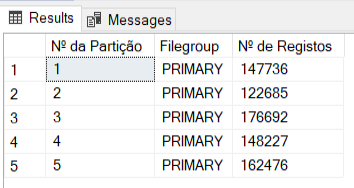
\includegraphics[width=0.45\textwidth]{../images/STEP2/Partitions.png}
\caption{Verification query result: record distribution across the 5 partitions}
\end{figure}

\section{Task 3: Indexes and Query Cost}

In this task, the impact of different indexing strategies on the \textit{Estimated Subtree Cost} of the following query was analysed. The query calculates the average price of new properties by locality in London:

\begin{lstlisting}[caption=Reference query for index analysis]
SELECT locality, AVG(price) AS average_new_property_price
FROM ShortPricePaidData2025
WHERE town = 'London'
AND OldNew = 'Y'
GROUP BY locality
ORDER BY average_new_property_price DESC;
\end{lstlisting}


\subsection{No Index - Baseline (SubTree Cost 10.0607)}

Without any auxiliary index, SQL Server performs a full \textit{Table Scan}, reading all 757\,816 records in the table before applying the \texttt{WHERE} filters. The absence of a selective access path forces the engine to scan the entire table.

\begin{figure}[htbp]
\centering
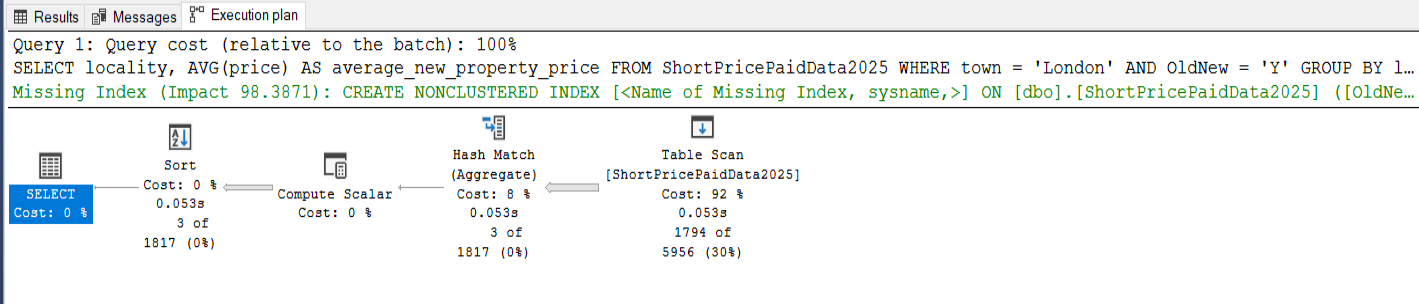
\includegraphics[width=\textwidth]{../images/STEP3/noindex.png}
\caption{Execution plan without index (Subtree Cost: 10.0607)}
\end{figure}

\pagebreak

\subsection{Simple Index on \texttt{town} (SubTree Cost 10.0595)}

\begin{lstlisting}[caption=Simple non-clustered index on town]
CREATE INDEX idx_town ON ShortPricePaidData2025(town);

-- Query to drop the respective index
DROP INDEX idx_town ON ShortPricePaidData2025;
\end{lstlisting}

With an index only on \texttt{town} on a heap table, the optimiser determines that a \textit{Non-Clustered Index Seek} followed by individual \textit{RID Lookups} into the heap for each matching row would be more expensive than simply scanning all data pages directly. As a result, SQL Server ignores the index and once again performs a full \textit{Table Scan}, leaving the cost virtually unchanged from the \textit{baseline}.

\begin{figure}[htbp]
\centering
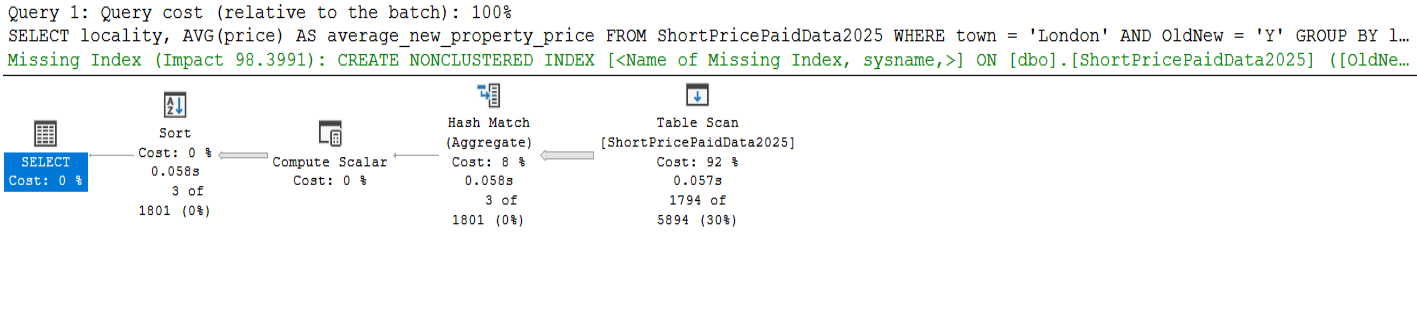
\includegraphics[width=\textwidth]{../images/STEP3/townidx.png}
\caption{Execution plan with index on \texttt{town} (Subtree Cost: 10.0595)}
\end{figure}

\subsection{Composite Index on \texttt{town} and \texttt{OldNew} (SubTree Cost 4.67951)}

\begin{lstlisting}[caption=Composite non-clustered index on town and OldNew]
CREATE INDEX idx_town_oldnew ON ShortPricePaidData2025(town, OldNew);

-- Query to drop the respective index
DROP INDEX idx_town_oldnew ON ShortPricePaidData2025;
\end{lstlisting}

By including \texttt{OldNew} in the index keys, SQL Server can filter simultaneously by \texttt{town = 'London'} and \texttt{OldNew = 'Y'} during the \textit{Seek}, substantially reducing the number of rows that require an \textit{RID Lookup (Heap)} into the data pages. The cost drops by $\approx$53\% compared to the \textit{baseline}.

\begin{figure}[htbp]
\centering
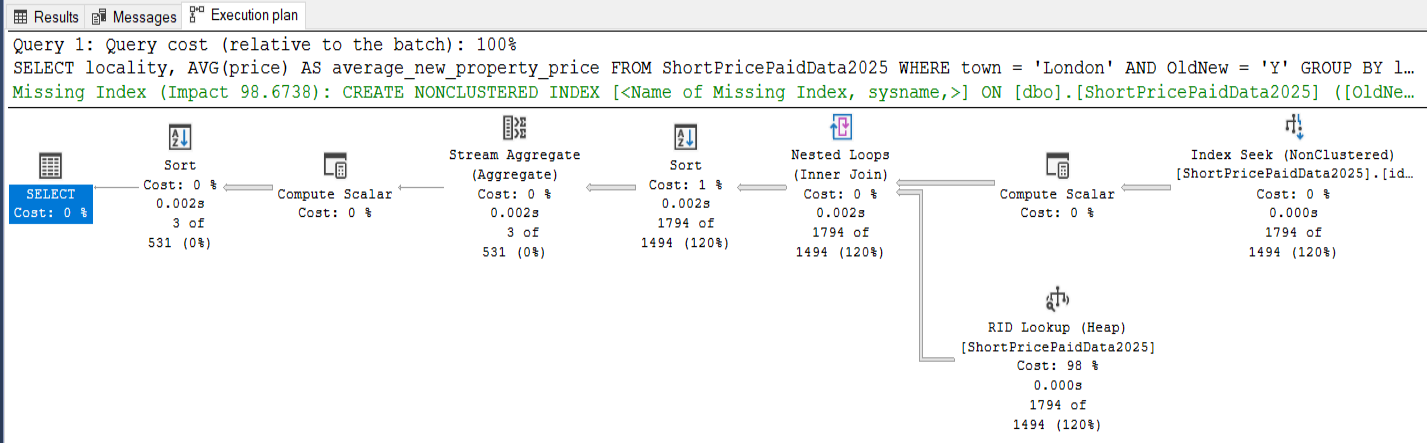
\includegraphics[width=\textwidth]{../images/STEP3/townoldnewidx.png}
\caption{Execution plan with index on (\texttt{town}, \texttt{OldNew}) (Subtree Cost: 4.67951)}
\end{figure}

\pagebreak

\subsection{Index with \texttt{locality} in the key and \texttt {INCLUDE} of \texttt{price} (SubTree Cost 0.0297144)}

\begin{lstlisting}[caption=Covering index with locality in the key and price in INCLUDE]
CREATE INDEX idx_query_cover
ON ShortPricePaidData2025(town, OldNew, locality)
INCLUDE(price);

-- Query to drop the respective index
DROP INDEX idx_query_cover ON ShortPricePaidData2025;
\end{lstlisting}

This index completely covers the query: the filter columns (\texttt{town}, \texttt{OldNew}), the grouping column (\texttt{locality}), and the calculated column (\texttt{price}) are all present in the index. SQL Server eliminates the \textit{RID Lookup}, resulting in a $\approx$99.7\% reduction compared to the \textit{baseline}. Furthermore, since \texttt{locality} is stored as an index key, the data returned by the \textit{Seek} is already ordered by \texttt{locality}, enabling a \textit{Stream Aggregate} without a pre-sort step. This index was suggested by SQL Server through the \textit{Missing Index} warning in the previous plans.

\begin{figure}[htbp]
\centering
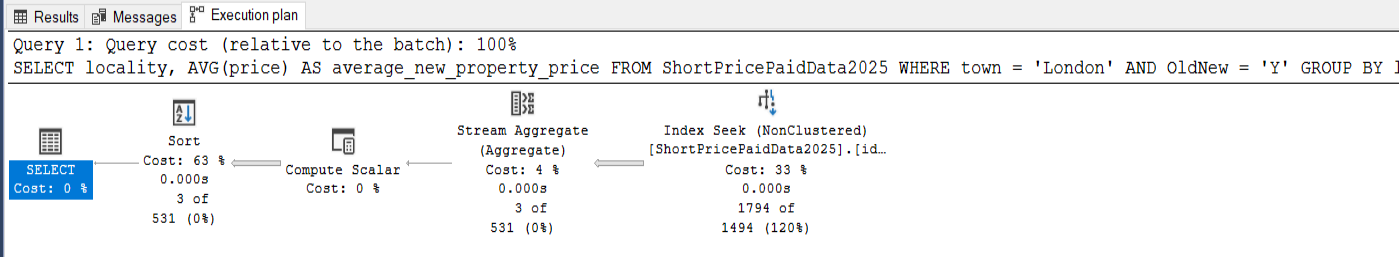
\includegraphics[width=\textwidth]{../images/STEP3/townoldnewlocalityidx.png}
\caption{Execution plan with covering index (\texttt{town}, \texttt{OldNew}, \texttt{locality}) INCLUDE(\texttt{price}) (Subtree Cost: 0.0297144)}
\end{figure}

\pagebreak

\subsection{Index with \texttt{locality} in \texttt{INCLUDE} (SubTree Cost 0.0656608)}

\begin{lstlisting}[caption=Optimal covering index with locality in INCLUDE]
CREATE INDEX idx_query_cover_2
ON ShortPricePaidData2025(town, OldNew)
INCLUDE(price, locality);

-- Query to drop the respective index
DROP INDEX idx_query_cover_2 ON ShortPricePaidData2025;
\end{lstlisting}

Moving \texttt{locality} to \texttt{INCLUDE} makes the leaf pages more compact, but it removes the ordering guarantee on \texttt{locality}. As a result, SQL Server must inject an additional \textit{Sort} operator before the \textit{Stream Aggregate} (to satisfy the \texttt{GROUP BY}) and a second \textit{Sort} for the \texttt{ORDER BY} clause. These two sort passes cause this configuration to cost $\approx$121\% \textbf{more} than \texttt{idx\_query\_cover}, making \texttt{idx\_query\_cover} (with \texttt{locality} as a key column) the optimal choice for this query.

\begin{figure}[htbp]
\centering
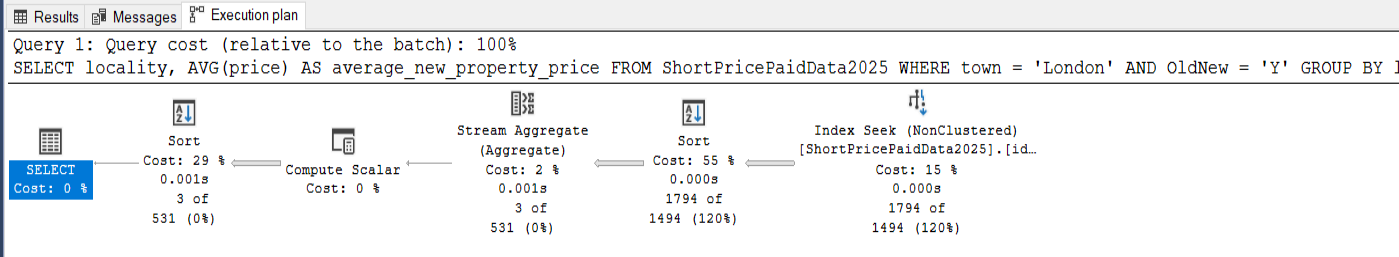
\includegraphics[width=\textwidth]{../images/STEP3/localityincludeidx.png}
\caption{Optimal execution plan with (\texttt{town}, \texttt{OldNew}) INCLUDE(\texttt{price}, \texttt{locality}) (Subtree Cost: 0.0656608)}
\end{figure}

\subsection{Comparative Summary}

\begin{table}[htbp]
\centering
\begin{tabular}{p{7.5cm}cc}
\toprule
\textbf{Configuration} & \textbf{Subtree Cost} & \textbf{Reduction} \\
\midrule
No index (baseline)
  & 10.0607   & - \\
\texttt{idx\_town} (\texttt{town})
  & 10.0595   & $\approx$0\% \\
\texttt{idx\_town\_oldnew} (\texttt{town}, \texttt{OldNew})
  & 4.67951   & $\approx$53\% \\
\texttt{idx\_query\_cover} (\texttt{town}, \texttt{OldNew}, \texttt{loc.}) \texttt{INC(price)}
  & 0.0297144 & $\approx$99.7\% \\
\texttt{idx\_query\_cover\_2} (\texttt{town}, \texttt{OldNew}) \texttt{INC(price, loc.)}
  & 0.0656608 & $\approx$99.3\% \\
\bottomrule
\end{tabular}
\caption{Comparison of the Estimated Subtree Cost by index configuration}
\end{table}

\section{Task 4: Study of Join and Aggregation Algorithms}

In this task, a comparative study of the \textit{Estimated Subtree Cost} was conducted for the query that identifies districts with an increase in average prices between 2024 and 2025. Combinations of aggregation algorithms (\textit{Hash} vs \textit{Order/Stream}) and join algorithms (\textit{Hash}, \textit{Merge}, \textit{Loop}) were tested using \textit{Query Hints}.

The analysed query identifies districts where the average price increased between 2024 and 2025:

\begin{lstlisting}[caption=Base query without hints (automatic optimiser choice)]
SELECT p24.district, p24.avg_price AS avg_2024, p25.avg_price AS avg_2025
FROM ( SELECT district, AVG(CAST(price AS BIGINT)) AS avg_price
       FROM ShortPricePaidData2024 GROUP BY district ) p24
JOIN ( SELECT district, AVG(CAST(price AS BIGINT)) AS avg_price
       FROM ShortPricePaidData2025 GROUP BY district ) p25
ON p24.district = p25.district
WHERE p25.avg_price > p24.avg_price;
\end{lstlisting}

\begin{figure}[htbp]
\centering
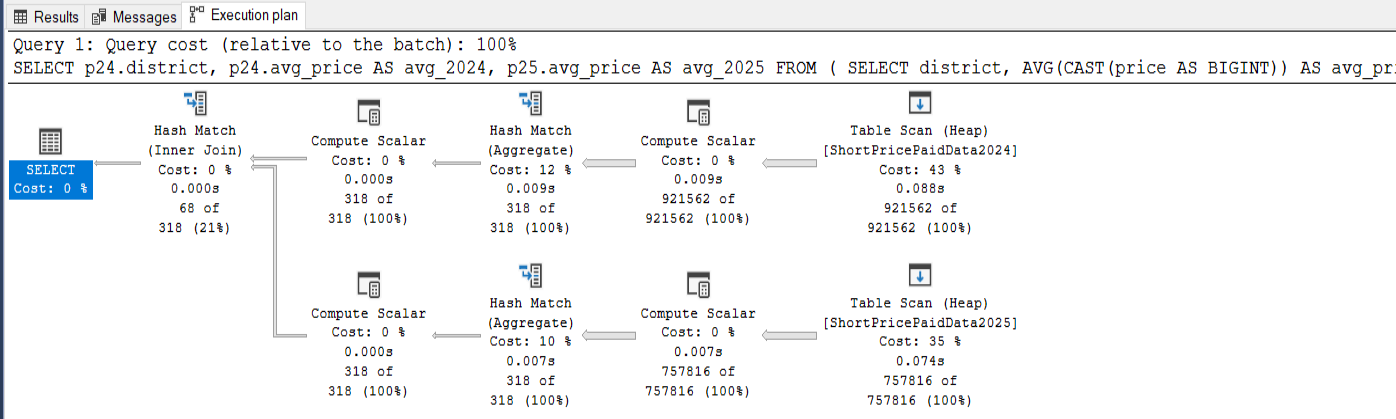
\includegraphics[width=\textwidth]{../images/STEP4/Original.png}
\caption{Execution plan without hints: the optimiser automatically chooses Hash Aggregate + Hash Join (Subtree Cost: 26.225)}
\end{figure}

Without any hint, the optimiser automatically chooses the Hash Aggregate + Hash Join combination, the most efficient for unordered data.

\subsection{Combinations with Hash Group (Hash Aggregation)}
In this configuration, SQL Server uses in-memory hash tables for grouping, which is efficient for unordered data.

\subsubsection{Hash Aggregate + Hash Join (Optimal Configuration)}
\begin{lstlisting}
SELECT p24.district, p24.avg_price AS avg_2024, p25.avg_price AS avg_2025 
FROM ( SELECT district, AVG(CAST(price AS BIGINT)) AS avg_price FROM ShortPricePaidData2024 GROUP BY district ) p24 
JOIN ( SELECT district, AVG(CAST(price AS BIGINT)) AS avg_price FROM ShortPricePaidData2025 GROUP BY district ) p25 
ON p24.district = p25.district 
WHERE p25.avg_price > p24.avg_price
OPTION (HASH GROUP, HASH JOIN);
\end{lstlisting}

\begin{figure}[htbp]
\centering
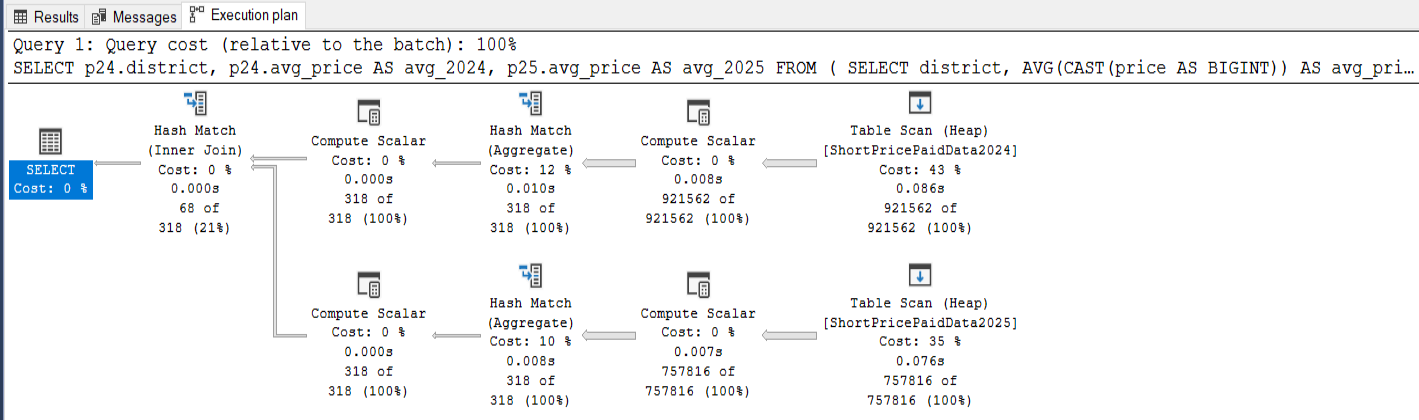
\includegraphics[width=\textwidth]{../images/STEP4/HashAggregateHashJoin.png}
\caption{Execution plan: Hash Aggregate + Hash Join (Subtree Cost: 26.225)}
\end{figure}

\textbf{Analysis (SubTree Cost 26.225) - Optimal Configuration:} This combination achieved the lowest estimated cost. Since the source tables are not pre-sorted by \textit{district}, the optimiser creates in-memory hash tables for both the grouping and the join phases.

\textbf{Why it performs better:} It completely avoids the \textit{Sort} operator. By using in-memory hash structures to map values, it maintains a linear scan cost instead of the $O(n \log n)$ cost associated with sorting large datasets.

\subsubsection{Hash Aggregate + Nested Loop Join}
\begin{lstlisting}
SELECT p24.district, p24.avg_price, p25.avg_price 
FROM (SELECT district, AVG(CAST(price AS BIGINT)) AS avg_price FROM ShortPricePaidData2024 GROUP BY district) p24 
JOIN (SELECT district, AVG(CAST(price AS BIGINT)) AS avg_price FROM ShortPricePaidData2025 GROUP BY district) p25 
ON p24.district = p25.district 
WHERE p25.avg_price > p24.avg_price
OPTION (HASH GROUP, LOOP JOIN);
\end{lstlisting}

\begin{figure}[htbp]
\centering
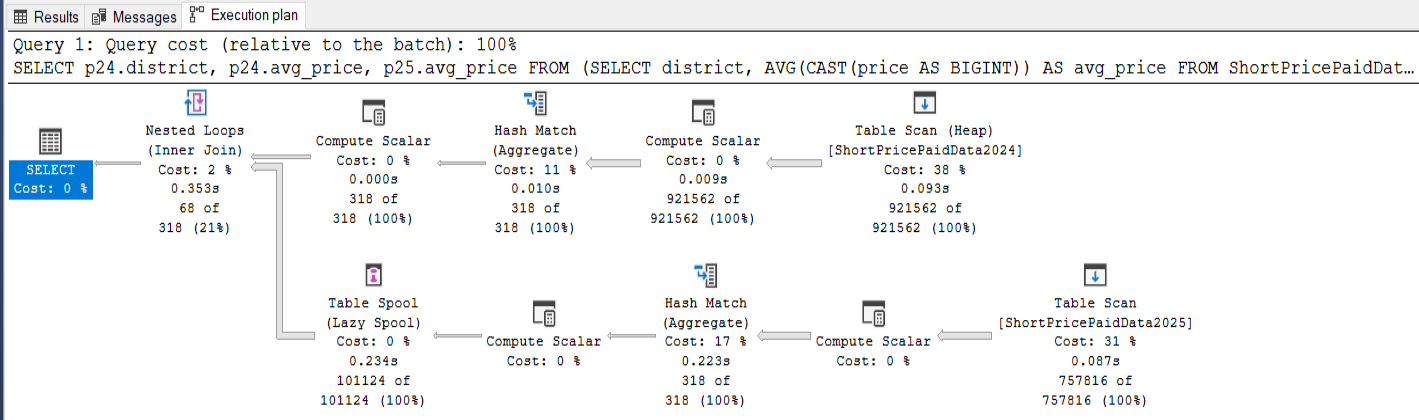
\includegraphics[width=\textwidth]{../images/STEP4/HashAggregateLoopJoin.png}
\caption{Execution plan: Hash Aggregate + Nested Loop Join (Subtree Cost: 29.3477)}
\end{figure}

\textbf{Analysis (SubTree Cost 29.3477) - Moderate Performance:} Grouping is performed efficiently via hash, but the join uses \textit{Nested Loop} logic.

\textbf{Plan detail:} The plan includes a \textit{Table Spool (Lazy Spool)} operator, used to cache the 2025 aggregation results and avoid a full re-scan of the sub-query for each row found in 2024. The overhead of managing this spool makes this combination slightly more expensive than a pure \textit{Hash Join}.

\pagebreak

\subsubsection{Hash Aggregate + Merge Join}
\begin{lstlisting}
SELECT p24.district, p24.avg_price, p25.avg_price 
FROM (SELECT district, AVG(CAST(price AS BIGINT)) AS avg_price FROM ShortPricePaidData2024 GROUP BY district) p24 
JOIN (SELECT district, AVG(CAST(price AS BIGINT)) AS avg_price FROM ShortPricePaidData2025 GROUP BY district) p25 
ON p24.district = p25.district 
WHERE p25.avg_price > p24.avg_price
OPTION (HASH GROUP, MERGE JOIN);
\end{lstlisting}

\begin{figure}[htbp]
\centering
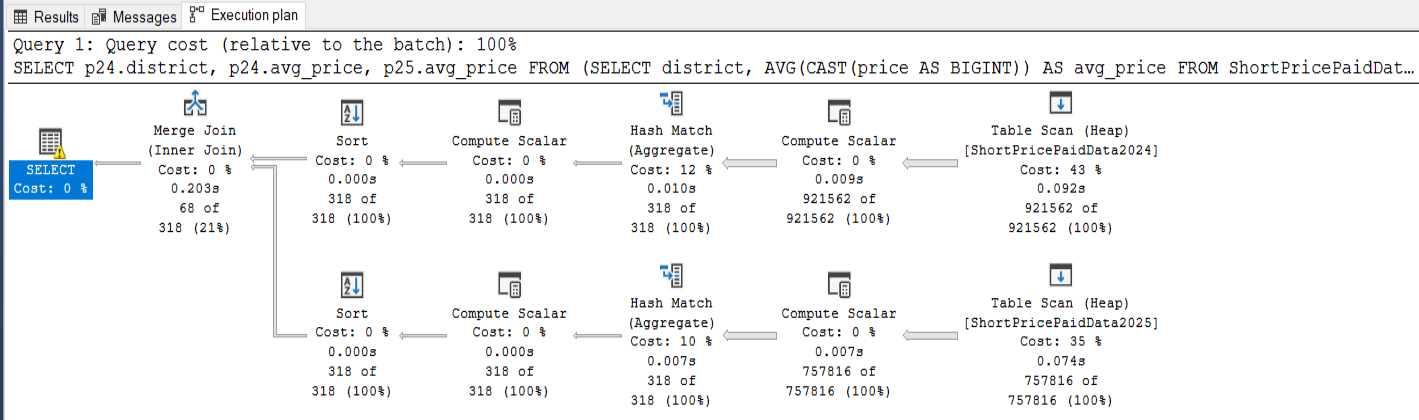
\includegraphics[width=\textwidth]{../images/STEP4/HashAggregateMergeJoin.png}
\caption{Execution plan: Hash Aggregate + Merge Join (Subtree Cost: 26.2311)}
\end{figure}


\textbf{Analysis (SubTree Cost 26.2311) - Poor Performance:} This combination creates a ``bottleneck'' effect. Although the initial grouping is fast via hash, the \textit{Merge Join} strictly requires sorted inputs.

\textbf{Why it performs worse:} The optimiser is forced to inject \textit{Sort} operators after the aggregation is complete, in order to prepare the data for the join. This transition from ``hashed'' data back to ``sorted'' data introduces unnecessary computational overhead.

\pagebreak

\subsection{Combinations with Order Group (Stream Aggregation)}
\textit{Order Group} requires that the data arrives at the aggregation operator already sorted by \textit{district}.


\subsubsection{Stream Aggregate + Hash Join}
\begin{lstlisting}
SELECT p24.district, p24.avg_price, p25.avg_price 
FROM (SELECT district, AVG(CAST(price AS BIGINT)) AS avg_price FROM ShortPricePaidData2024 GROUP BY district) p24 
JOIN (SELECT district, AVG(CAST(price AS BIGINT)) AS avg_price FROM ShortPricePaidData2025 GROUP BY district) p25 
ON p24.district = p25.district 
WHERE p25.avg_price > p24.avg_price
OPTION (ORDER GROUP, HASH JOIN);
\end{lstlisting}

\begin{figure}[htbp]
\centering
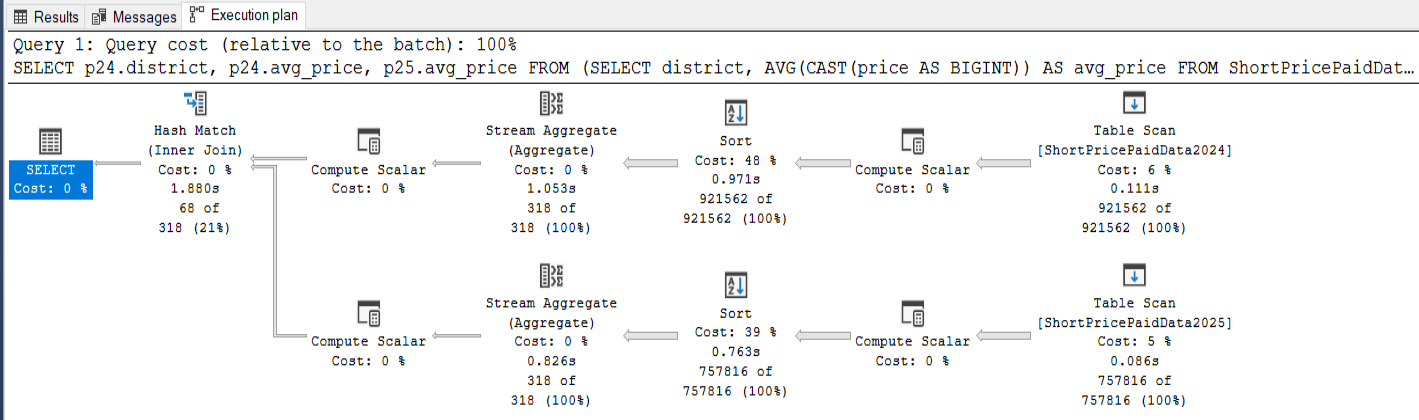
\includegraphics[width=\textwidth]{../images/STEP4/StreamAgregateHashJoin.png}
\caption{Execution plan: Stream Aggregate + Hash Join (Subtree Cost: 173.47)}
\end{figure}

\textbf{Analysis (SubTree Cost 173.47) - Poor Performance:} By forcing \texttt{ORDER GROUP}, SQL Server must ensure that the data arrives at the aggregation operator already sorted by \textit{district}.

\textbf{Plan detail:} The plan shows heavy \textit{Sort} operators immediately after the \textit{Table Scans (Heap)}. As these sorts operate on the raw data (hundreds of thousands of rows), the \textit{Sort} cost far outweighs any benefit provided by the subsequent \textit{Hash Join}.

\pagebreak

\subsubsection{Stream Aggregate + Merge Join (Worst Case)}
\begin{lstlisting}
SELECT p24.district, p24.avg_price AS avg_2024, p25.avg_price AS avg_2025 
FROM ( SELECT district, AVG(CAST(price AS BIGINT)) AS avg_price FROM ShortPricePaidData2024 GROUP BY district ) p24 
JOIN ( SELECT district, AVG(CAST(price AS BIGINT)) AS avg_price FROM ShortPricePaidData2025 GROUP BY district ) p25 
ON p24.district = p25.district 
WHERE p25.avg_price > p24.avg_price
OPTION (ORDER GROUP, MERGE JOIN);
\end{lstlisting}

\begin{figure}[htbp]
\centering
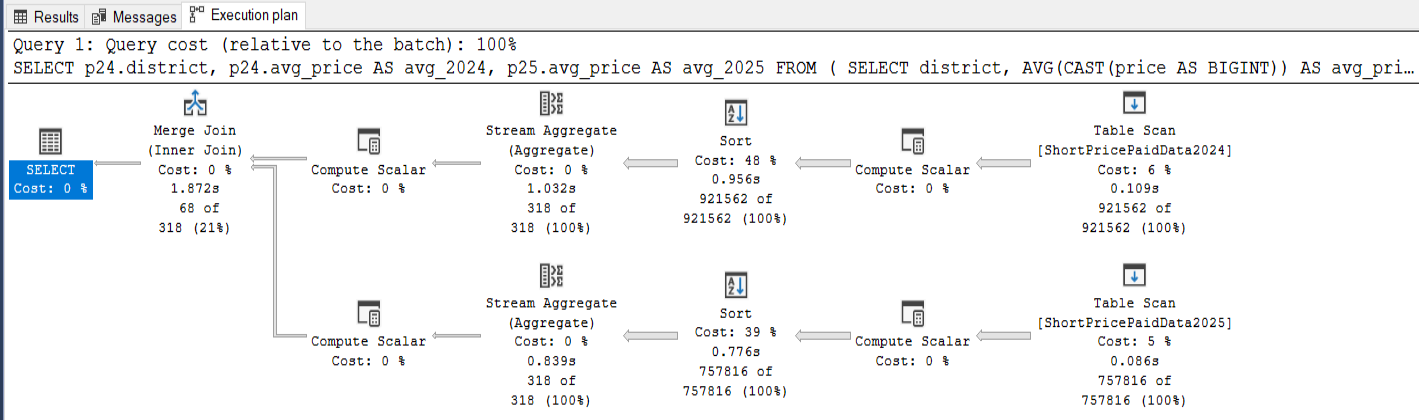
\includegraphics[width=\textwidth]{../images/STEP4/StreamAgregateMergeJoin.png}
\caption{Execution plan: Stream Aggregate + Merge Join (Subtree Cost: $\approx$173.448)}
\end{figure}

\textbf{Analysis (SubTree Cost 173.448) - Worst Case:} This combination resulted in the highest estimated cost. Both \textit{Stream Aggregate} and \textit{Merge Join} require sorted data.

\textbf{Conclusion:} This is the ``Worst Case'' for data without an index. The engine must perform massive sorts on both tables. Although the join and aggregation logic is very efficient once the data is sorted, the \textit{Sort} operator becomes the dominant resource consumer in the entire query.

\pagebreak

\subsubsection{Stream Aggregate + Loop Join}
\begin{lstlisting}
SELECT p24.district, p24.avg_price, p25.avg_price 
FROM (SELECT district, AVG(CAST(price AS BIGINT)) AS avg_price FROM ShortPricePaidData2024 GROUP BY district) p24 
JOIN (SELECT district, AVG(CAST(price AS BIGINT)) AS avg_price FROM ShortPricePaidData2025 GROUP BY district) p25 
ON p24.district = p25.district 
WHERE p25.avg_price > p24.avg_price
OPTION (ORDER GROUP, LOOP JOIN);
\end{lstlisting}

\begin{figure}[htbp]
\centering
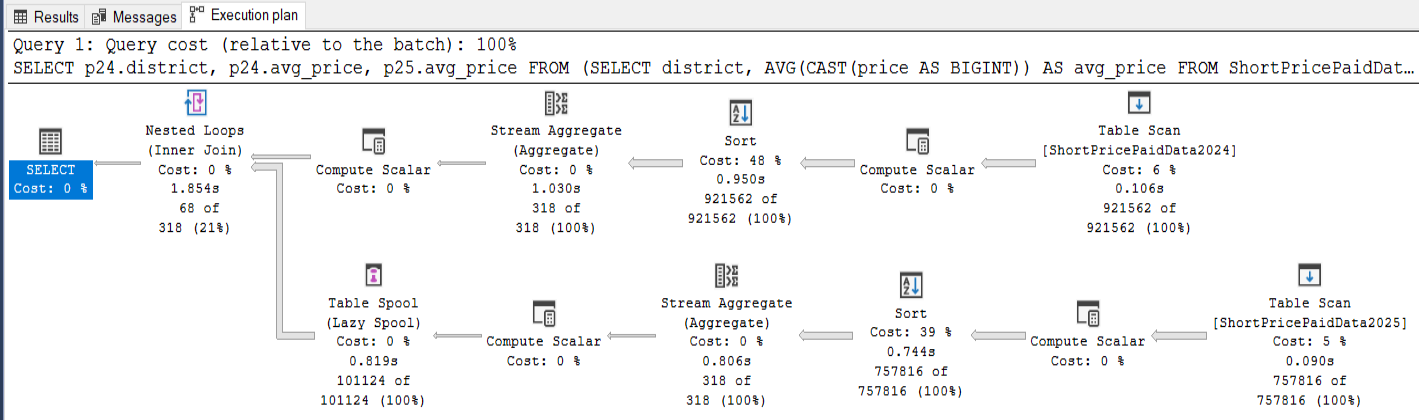
\includegraphics[width=\textwidth]{../images/STEP4/StreamAgregateLoopJoin.png}
\caption{Execution plan: Stream Aggregate + Nested Loop Join (Subtree Cost: 173.994)}
\end{figure}

\textbf{Analysis (SubTree Cost 173.994) - Very Poor Performance:} Similar to the previous case, the cost is inflated by the initial sort required by the \textit{Stream Aggregate}. Adding a \textit{Nested Loop} over sorted data provides no performance benefit in this context.

\textbf{Additional note:} The engine cannot leverage the existing sort order to execute a faster join, unlike what would happen with a \textit{Merge Join}, where the pre-sorted data would be reused by the join logic.

\pagebreak

\section{Task 5: Query Tuning}

The original query was rewritten to improve performance in identifying properties sold in both years, using the \texttt{EXISTS} clause.

\begin{lstlisting}[caption=Default Query]
WITH p24 AS ( 
SELECT DISTINCT county, PAON, street, town 
FROM ShortPricePaidData2024 
), 
p25 AS ( 
SELECT DISTINCT county, PAON, street, town 
FROM ShortPricePaidData2025 
) 
SELECT p24.county, COUNT(*) AS properties_sold_both_years 
FROM p24 JOIN p25 
ON p24.county = p25.county 
AND p24.PAON = p25.PAON 
AND p24.street = p25.street 
AND p24.town = p25.town 
GROUP BY p24.county;
\end{lstlisting}

\begin{figure}[htbp]
\centering
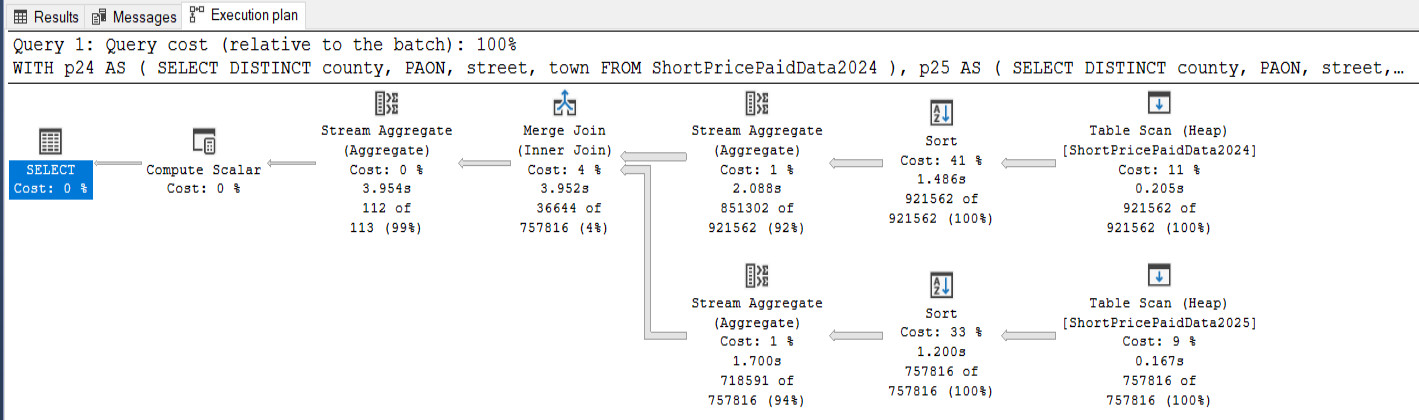
\includegraphics[width=\textwidth]{../images/STEP5/default.png}
\caption{Execution plan of the default query \textbf{(Estimated Subtree Cost: 102.124)}}
\end{figure}

The default query materialises and fully joins deduplicated sets, processing all matching rows (including duplicates), whereas the optimized version uses \texttt{EXISTS} (a semi-join) to match a single instance of each 2024 row.

\pagebreak

\begin{lstlisting}[caption=Optimised Query \textbf{(Estimated Subtree Cost: 48.8274)}]
SELECT p24.county, COUNT(DISTINCT p24.PAON + p24.street + p24.town) AS properties_sold_both_years
FROM ShortPricePaidData2024 p24
WHERE EXISTS (
    SELECT 1 FROM ShortPricePaidData2025 p25
    WHERE p24.county = p25.county AND p24.PAON = p25.PAON 
      AND p24.street = p25.street AND p24.town = p25.town
)
GROUP BY p24.county
ORDER BY p24.county;
\end{lstlisting}

\begin{figure}[htbp]
\centering
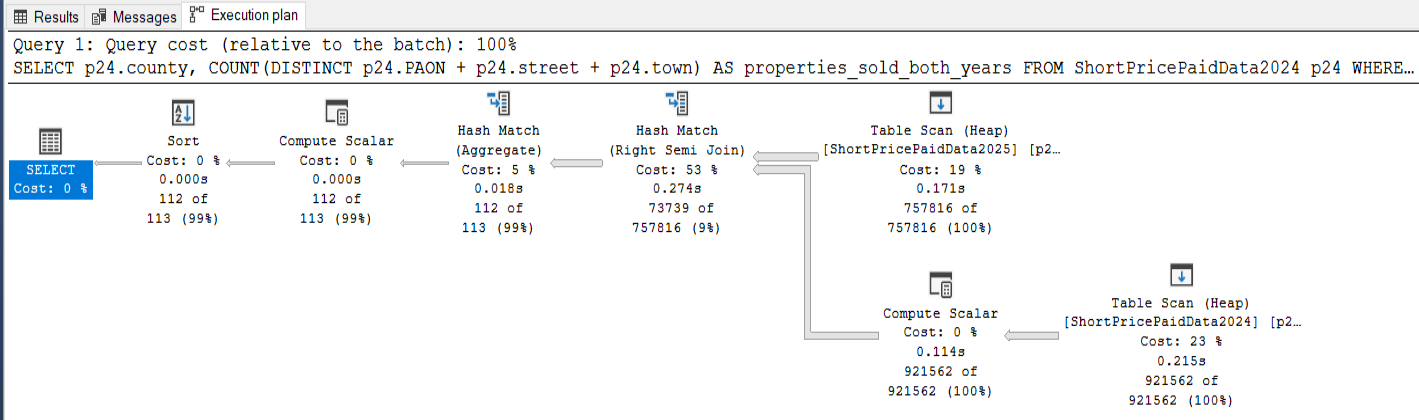
\includegraphics[width=\textwidth]{../images/STEP5/optimised.png}
\caption{Execution plan of the optimised query \textbf{(Estimated Subtree Cost: 48.8274)}}
\end{figure}

\textbf{Justification:} \texttt{EXISTS} enables a \textit{Semi-Join}, where processing stops as soon as the first match is found in 2025 for each 2024 record, reducing I/O load compared to a traditional \textit{Join}.

\section{Task 6: Transactions and Isolation Levels}

Demonstration of how isolation levels affect the correctness of analytical queries running concurrently with insertions. Three scenarios are presented, each executed across two concurrent terminals.

\subsection{Scenario 1 - READ UNCOMMITTED: Dirty Read and Non-Repeatable Read}

\textbf{Step 1 [Terminal 1]:} Start an insertion but do not commit it.

\begin{lstlisting}
BEGIN TRANSACTION;
INSERT INTO ShortPricePaidData2025 (
    TransactionID, Price, DateOfTransfer, Postcode,
    PropertyType, OldNew, PAON, Street, Locality, Town, District, County
)
VALUES (NEWID(), 5000000, GETDATE(), 'SW1A 1AA', 'D', 'Y',
        '1', 'Downing St', 'Westminster', 'London', 'London', 'Greater London');
\end{lstlisting}

\textbf{Step 2 [Terminal 2]:} Read the data under \texttt{READ UNCOMMITTED}. The average price for \texttt{Westminster} is drastically inflated by the uncommitted £5\,000\,000 row.

\begin{lstlisting}
SET TRANSACTION ISOLATION LEVEL READ UNCOMMITTED;
BEGIN TRANSACTION;
SELECT locality, AVG(price) AS average_new_property_price
FROM ShortPricePaidData2025
WHERE town = 'London' AND OldNew = 'Y'
GROUP BY locality;
\end{lstlisting}

\textbf{Step 3 [Terminal 1]:} Roll back the insertion, the uncommitted row never existed.

\begin{lstlisting}
ROLLBACK TRANSACTION;
\end{lstlisting}

\textbf{Step 4 [Terminal 2]:} Re-read the data. The \texttt{Westminster} average now returns to its true value, demonstrating a \textit{Dirty Read} followed by a \textit{Non-Repeatable Read} within the same transaction.

\begin{lstlisting}
SELECT locality, AVG(price) AS average_new_property_price
FROM ShortPricePaidData2025
WHERE town = 'London' AND OldNew = 'Y'
GROUP BY locality;
COMMIT TRANSACTION;
\end{lstlisting}

\texttt{READ UNCOMMITTED} does not prevent \textit{Dirty Reads} or \textit{Non-Repeatable Reads}. A transaction can read data that has been written but not yet committed by another transaction.

\subsection{Scenario 2 - READ COMMITTED: Dirty Read Prevention}

\textbf{Step 1 [Terminal 1]:} Start an update but do not commit it.

\begin{lstlisting}
BEGIN TRANSACTION;
UPDATE ShortPricePaidData2025
SET Price = Price * 2
WHERE Locality = 'LEYTON' AND OldNew = 'Y';
\end{lstlisting}

\textbf{Step 2 [Terminal 2]:} Attempt to read under \texttt{READ COMMITTED}. The query blocks until Terminal 1 releases its locks, or reads only previously committed values, the doubled prices are never visible.

\begin{lstlisting}
SET TRANSACTION ISOLATION LEVEL READ COMMITTED;
BEGIN TRANSACTION;
SELECT locality, AVG(price) AS average_new_property_price
FROM ShortPricePaidData2025
WHERE town = 'London' AND OldNew = 'Y'
GROUP BY locality;
\end{lstlisting}

\textbf{Step 3 [Terminal 1]:} Commit the update, releasing the locks.

\begin{lstlisting}
COMMIT TRANSACTION;
\end{lstlisting}

\textbf{Step 4 [Terminal 2]:} Re-read the data. The query now reflects the committed doubled prices for \texttt{Leyton}, illustrating a \textit{Non-Repeatable Read} that \texttt{READ COMMITTED} does not prevent.

\begin{lstlisting}
SELECT locality, AVG(price) AS average_new_property_price
FROM ShortPricePaidData2025
WHERE town = 'London' AND OldNew = 'Y'
GROUP BY locality;
COMMIT TRANSACTION;
\end{lstlisting}

\texttt{READ COMMITTED} ensures that only committed data is ever visible, preventing \textit{Dirty Reads}. It does not, however, prevent \textit{Non-Repeatable Reads}.

\subsection{Scenario 3 - SERIALIZABLE: Maximum Isolation}

\textbf{Step 1 [Terminal 2]:} Begin a read transaction under \texttt{SERIALIZABLE}. Range locks are acquired on the relevant rows in \texttt{ShortPricePaidData2025}.

\begin{lstlisting}
SET TRANSACTION ISOLATION LEVEL SERIALIZABLE;
BEGIN TRANSACTION;
SELECT locality, AVG(price) AS average_new_property_price
FROM ShortPricePaidData2025
WHERE town = 'London' AND OldNew = 'Y'
GROUP BY locality;
\end{lstlisting}

\textbf{Step 2 [Terminal 1]:} Attempt to insert a new London property. The statement blocks because the range is locked by Terminal 2's transaction.

\begin{lstlisting}
INSERT INTO ShortPricePaidData2025 (
    TransactionID, Price, DateOfTransfer, Postcode,
    PropertyType, OldNew, PAON, Street, Locality, Town, District, County
)
VALUES (NEWID(), 1000000, GETDATE(), 'E1 6AN', 'T', 'Y',
        '10', 'Brick Ln', 'Spitalfields', 'London', 'London', 'Greater London');
\end{lstlisting}

\textbf{Step 3 [Terminal 2]:} Re-read the data. The result is identical to Step 1, the blocked insertion from Terminal 1 has not affected the dataset. Committing releases the locks.

\begin{lstlisting}
SELECT locality, AVG(price) AS average_new_property_price
FROM ShortPricePaidData2025
WHERE town = 'London' AND OldNew = 'Y'
GROUP BY locality;
COMMIT TRANSACTION;
\end{lstlisting}

\texttt{SERIALIZABLE} is the strictest isolation level. It places range locks on the scanned data, preventing any concurrent insertions or modifications to that range until the transaction completes, thus eliminating \textit{Dirty Reads}, \textit{Non-Repeatable Reads}, and \textit{Phantom Reads}.

\section*{Declaration}
We used Gemini to validate SQL Server syntax during the development of this report. Additionally, we used GitHub Copilot (GPT-5 mini) to assist editing LaTeX formatting.

\end{document}